\documentclass[11pt,a4paper]{scrartcl}
\usepackage[a4paper, top=15mm, bottom=15mm, left=18mm, right=18mm]{geometry}
\usepackage{lmodern}
\usepackage[T1]{fontenc}
\usepackage[utf8]{inputenc}
\usepackage[ngerman]{babel}
\usepackage{microtype}
\usepackage{parskip}
\usepackage{graphicx}
\usepackage{float}
\usepackage{enumitem}
\usepackage{caption}
\usepackage[hidelinks]{hyperref}

\captionsetup{font=small, labelfont=bf, skip=4pt}
\setlist{nosep, leftmargin=1.5em}
\pagestyle{empty}

\begin{document}

\begin{center}
  {\Large\bfseries RocksDB unter Speicherbeschränkung -- Ergebnisse}\\[4pt]
  {\normalsize 256\,MB RAM, 1 CPU, kein Swap\enspace$\vert$\enspace
   100 Durchläufe (58 ok, 42 OOM)\enspace$\vert$\enspace
   Workload: \texttt{readwhilewriting}}
\end{center}

\bigskip

% ── Plot 1 ────────────────────────────────────────────────────────────────────
\begin{figure}[H]
  \centering
  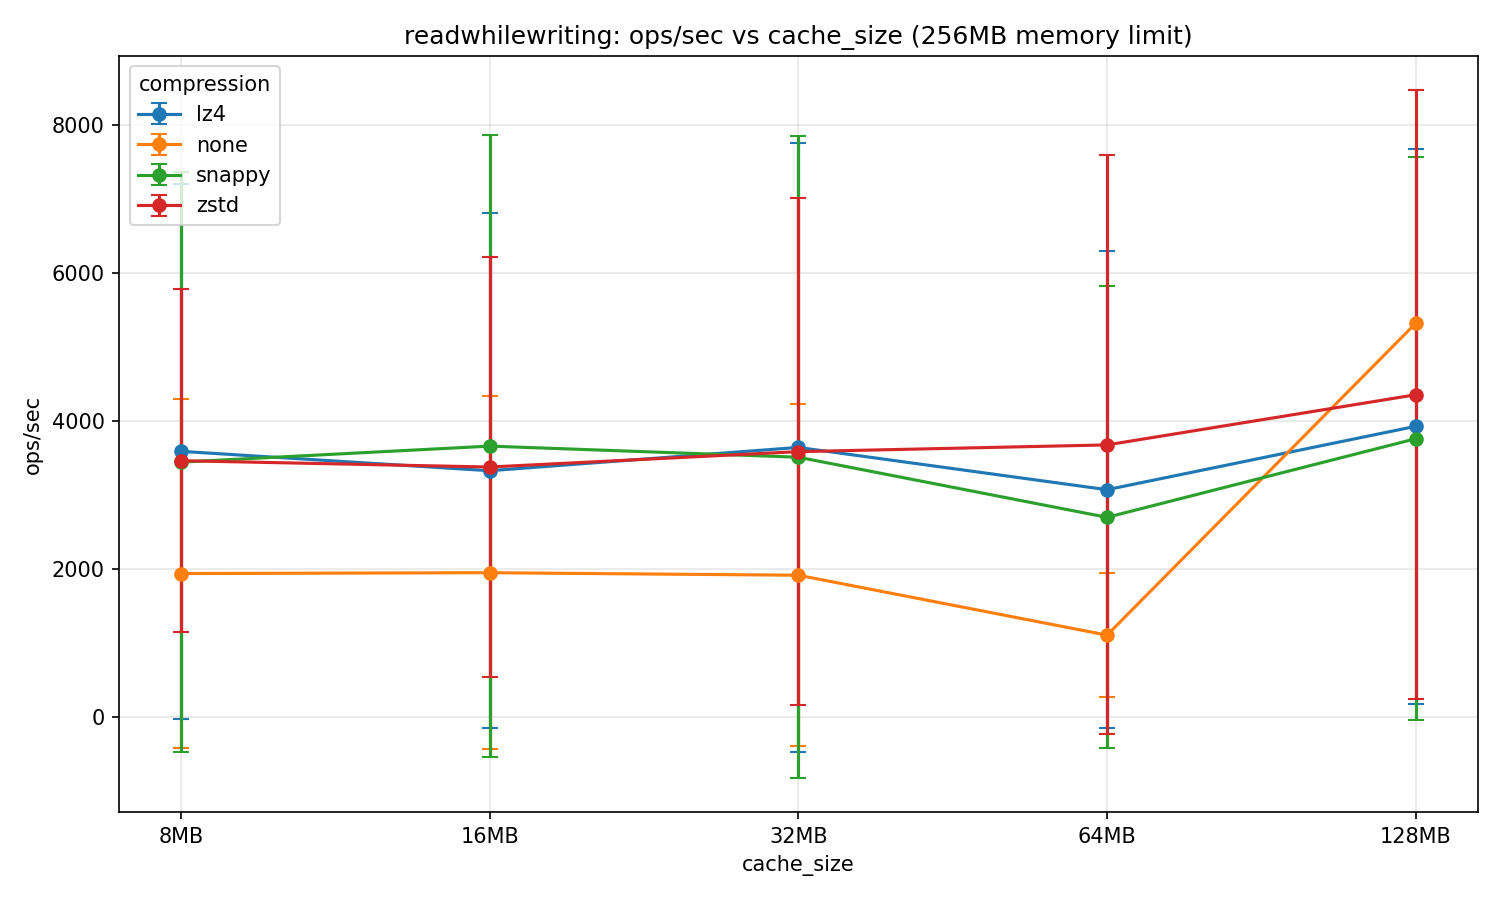
\includegraphics[width=0.95\textwidth]{parsed/plot_readwhilewriting_ops_vs_cache_size.png}
  \caption{Durchsatz (ops/sec) vs.\ Block-Cache-Größe, nach Kompressionsverfahren}
\end{figure}

\begin{itemize}
  \item Kompression macht einen riesigen Unterschied -- ohne Kompression nur halb so viel Durchsatz
  \item zstd, lz4 und snappy liegen nah beieinander; alle deutlich besser als \glqq none\grqq
  \item Die großen Fehlerbalken kommen daher, dass verschiedene \texttt{write\_buffer\_size}-Werte gemittelt werden -- kleine Puffer (4\,MB) sind viel schneller als große (16--32\,MB)
  \item Cache-Größe allein beeinflusst den Durchsatz weniger als erwartet
\end{itemize}

\bigskip

% ── Plot 2 ────────────────────────────────────────────────────────────────────
\begin{figure}[H]
  \centering
  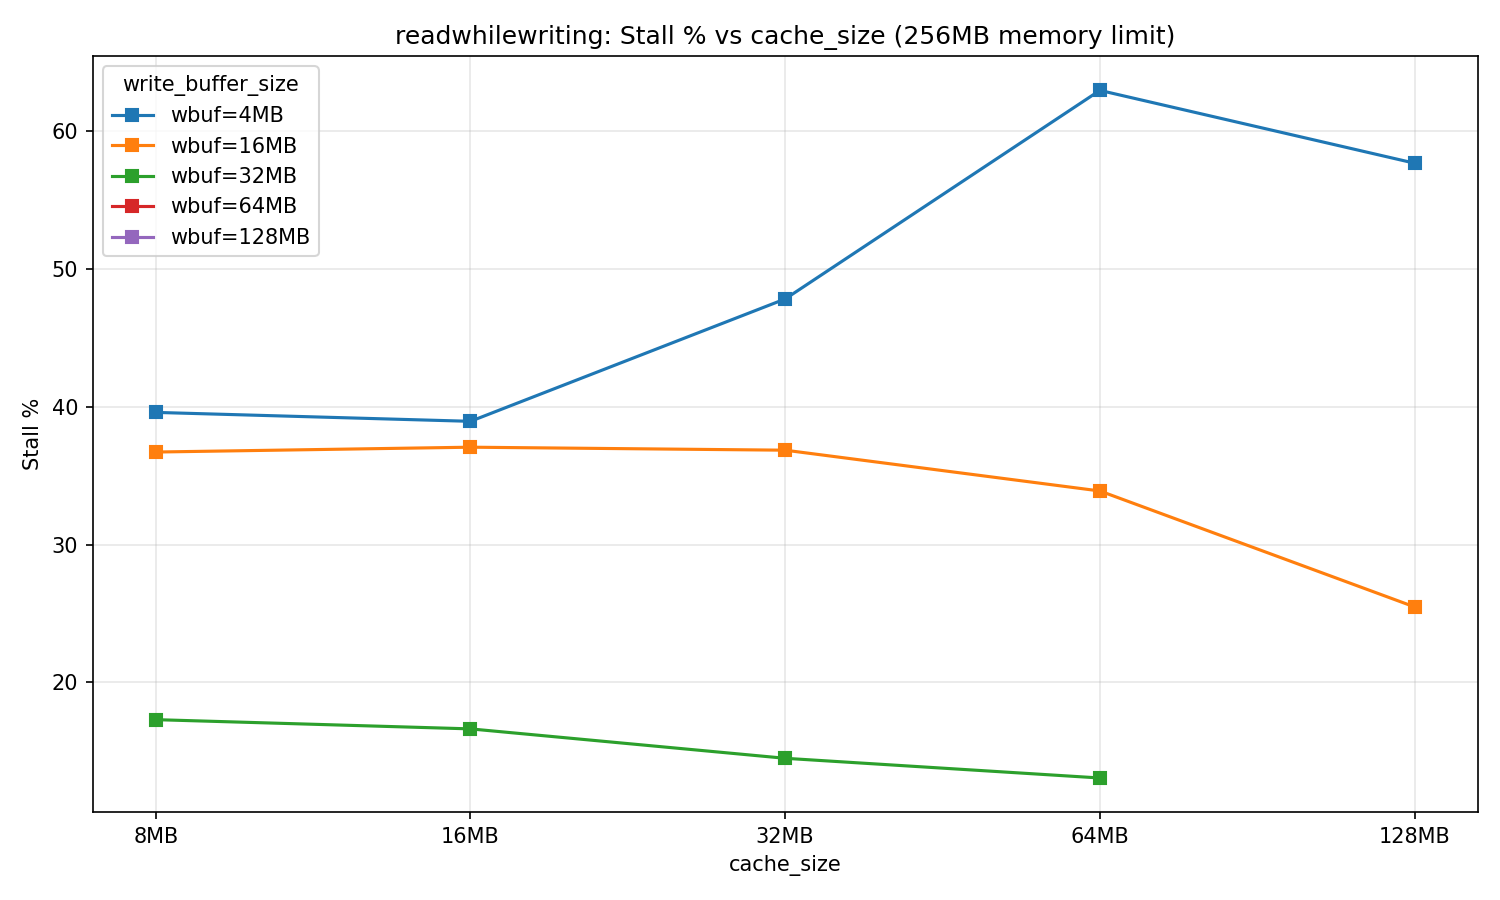
\includegraphics[width=0.95\textwidth]{parsed/plot_readwhilewriting_stalls_vs_cache_size.png}
  \caption{Write-Stall-Anteil (\%) vs.\ Block-Cache-Größe, nach Schreibpuffergröße}
\end{figure}

\begin{itemize}
  \item Kleiner Schreibpuffer (4\,MB) = höchster Stall-Anteil (40--63\,\%), \emph{aber} trotzdem höchster Durchsatz
  \item Erklärung: viele kleine Flushes gehen schneller durch als wenige große unter Speicherdruck
  \item Großer Schreibpuffer (32\,MB) = nur 15\,\% Stall, aber jeder einzelne Flush ist teuer $\rightarrow$ niedrigerer Gesamtdurchsatz
  \item 64\,MB und 128\,MB fehlen im Plot -- die sind fast alle OOM-gekillt worden
  \item Stall = RocksDB blockiert Schreibzugriffe $\rightarrow$ in NebulaStream würde das die ganze Pipeline aufstauen
\end{itemize}

\newpage

% ── Plot 3 ────────────────────────────────────────────────────────────────────
\begin{figure}[H]
  \centering
  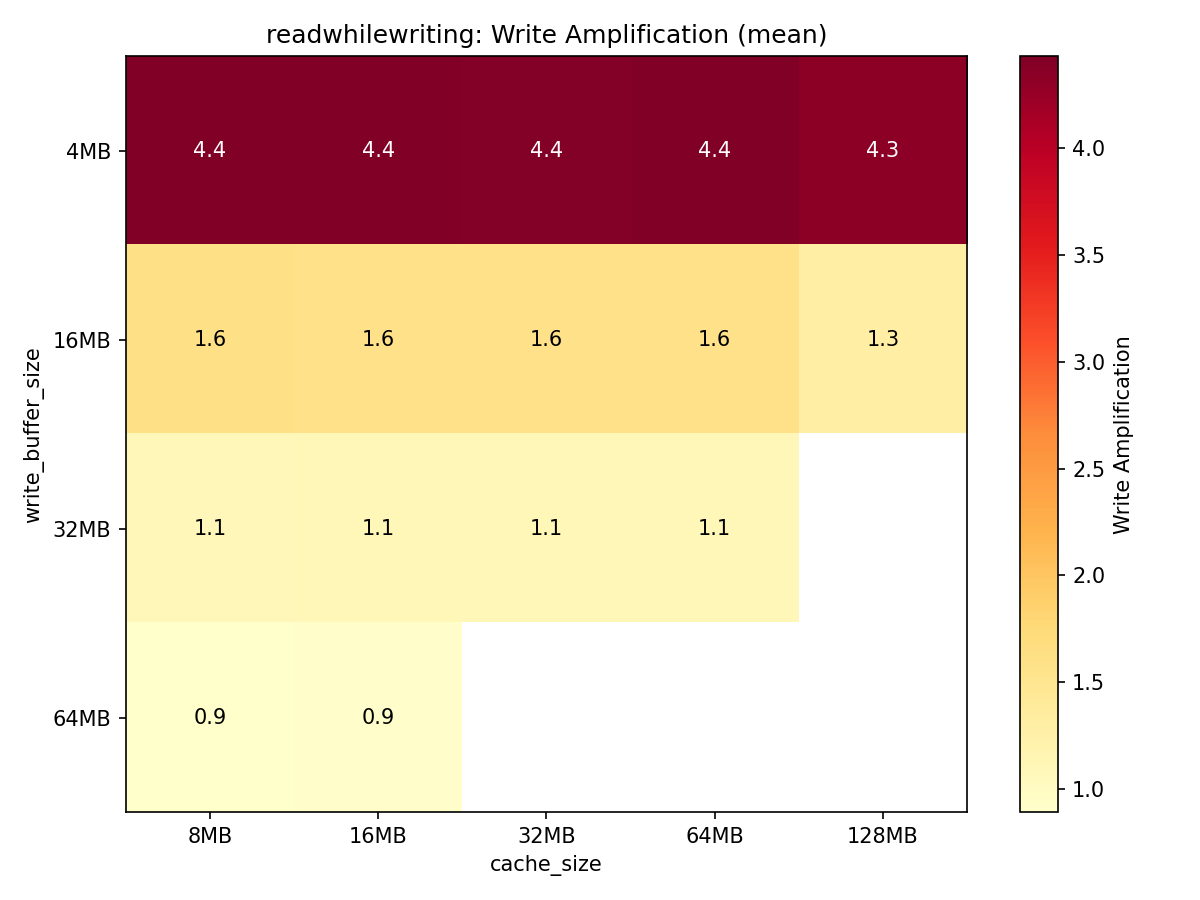
\includegraphics[width=0.75\textwidth]{parsed/plot_readwhilewriting_write_amp_heatmap.png}
  \caption{Schreibverstärkung (Write Amplification) -- Schreibpuffer $\times$ Cache-Größe}
\end{figure}

\begin{itemize}
  \item Write Amplification = wie viel mehr auf die Platte geschrieben wird als eigentlich nötig
  \item 4\,MB Schreibpuffer $\rightarrow$ 4,4$\times$ Write Amp (flusht sehr oft $\rightarrow$ viel Compaction)
  \item 32\,MB Schreibpuffer $\rightarrow$ 1,1$\times$ (fast optimal, flusht seltener)
  \item 64\,MB $\rightarrow$ 0,9$\times$ (am besten), aber stürzt meistens ab (OOM)
  \item Cache-Größe hat kaum Einfluss auf die Write Amplification -- das ist rein vom Schreibpuffer getrieben
  \item Hohe Write Amp = SD-Karte auf Edge-Gerät nutzt sich schneller ab
\end{itemize}

\bigskip

% ── Zusammenfassung ───────────────────────────────────────────────────────────
\begin{center}
\rule{0.8\textwidth}{0.4pt}
\end{center}

\subsection*{Was heißt das zusammen?}

\begin{itemize}
  \item Es gibt einen \textbf{17-fachen Leistungsunterschied} zwischen bester und schlechtester Konfiguration -- auf derselben Hardware
  \item Beste Kombination: kleiner Schreibpuffer (4\,MB) + Kompression (lz4/zstd) $\rightarrow$ ca.\ 9.000~ops/sec
  \item Schlechteste: mittlerer Schreibpuffer (16\,MB) + keine Kompression $\rightarrow$ ca.\ 500~ops/sec
  \item Ab 64\,MB Schreibpuffer ist das Gerät nicht mehr nutzbar (OOM)
  \item Kompression ist auf Edge-Hardware \textbf{Pflicht}, nicht optional
  \item Write-Stalls sind ein echtes Problem für Streamverarbeitung -- im Schnitt 34\,\% der Zeit blockiert
\end{itemize}

\subsection*{Aber:}

\begin{itemize}
  \item Bisher nur 1 Workload, 3 von 5 Parametern, synthetische Datengrößen
  \item Ergebnisse zeigen die \emph{Richtung}, exakte Zahlen sind nicht 1:1 auf NebulaStream übertragbar
  \item Nächster Schritt: mehr Workloads + vollständiger Parameter-Sweep
\end{itemize}

\end{document}
